\documentclass[11pt, oneside]{article} 
\usepackage{geometry}
\geometry{letterpaper} 
\usepackage{graphicx}
	
\usepackage{amssymb}
\usepackage{amsmath}
\usepackage{parskip}
\usepackage{color}
\usepackage{hyperref}

\graphicspath{{/Users/telliott/Github-math/figures/}}
% \begin{center} \includegraphics [scale=0.4] {gauss3.png} \end{center}

\title{Acheson G163}
\date{}

\begin{document}
\maketitle
\Large

%[my-super-duper-separator]

Acheson presents this problem (though he does not show the solution).  The algebra defeated me for quite a long time, but I finally got it.

We are given only the radii of the small circles, $a,b$ and $c$, and are asked to find $r$, which I have written as $R$.

\begin{center} 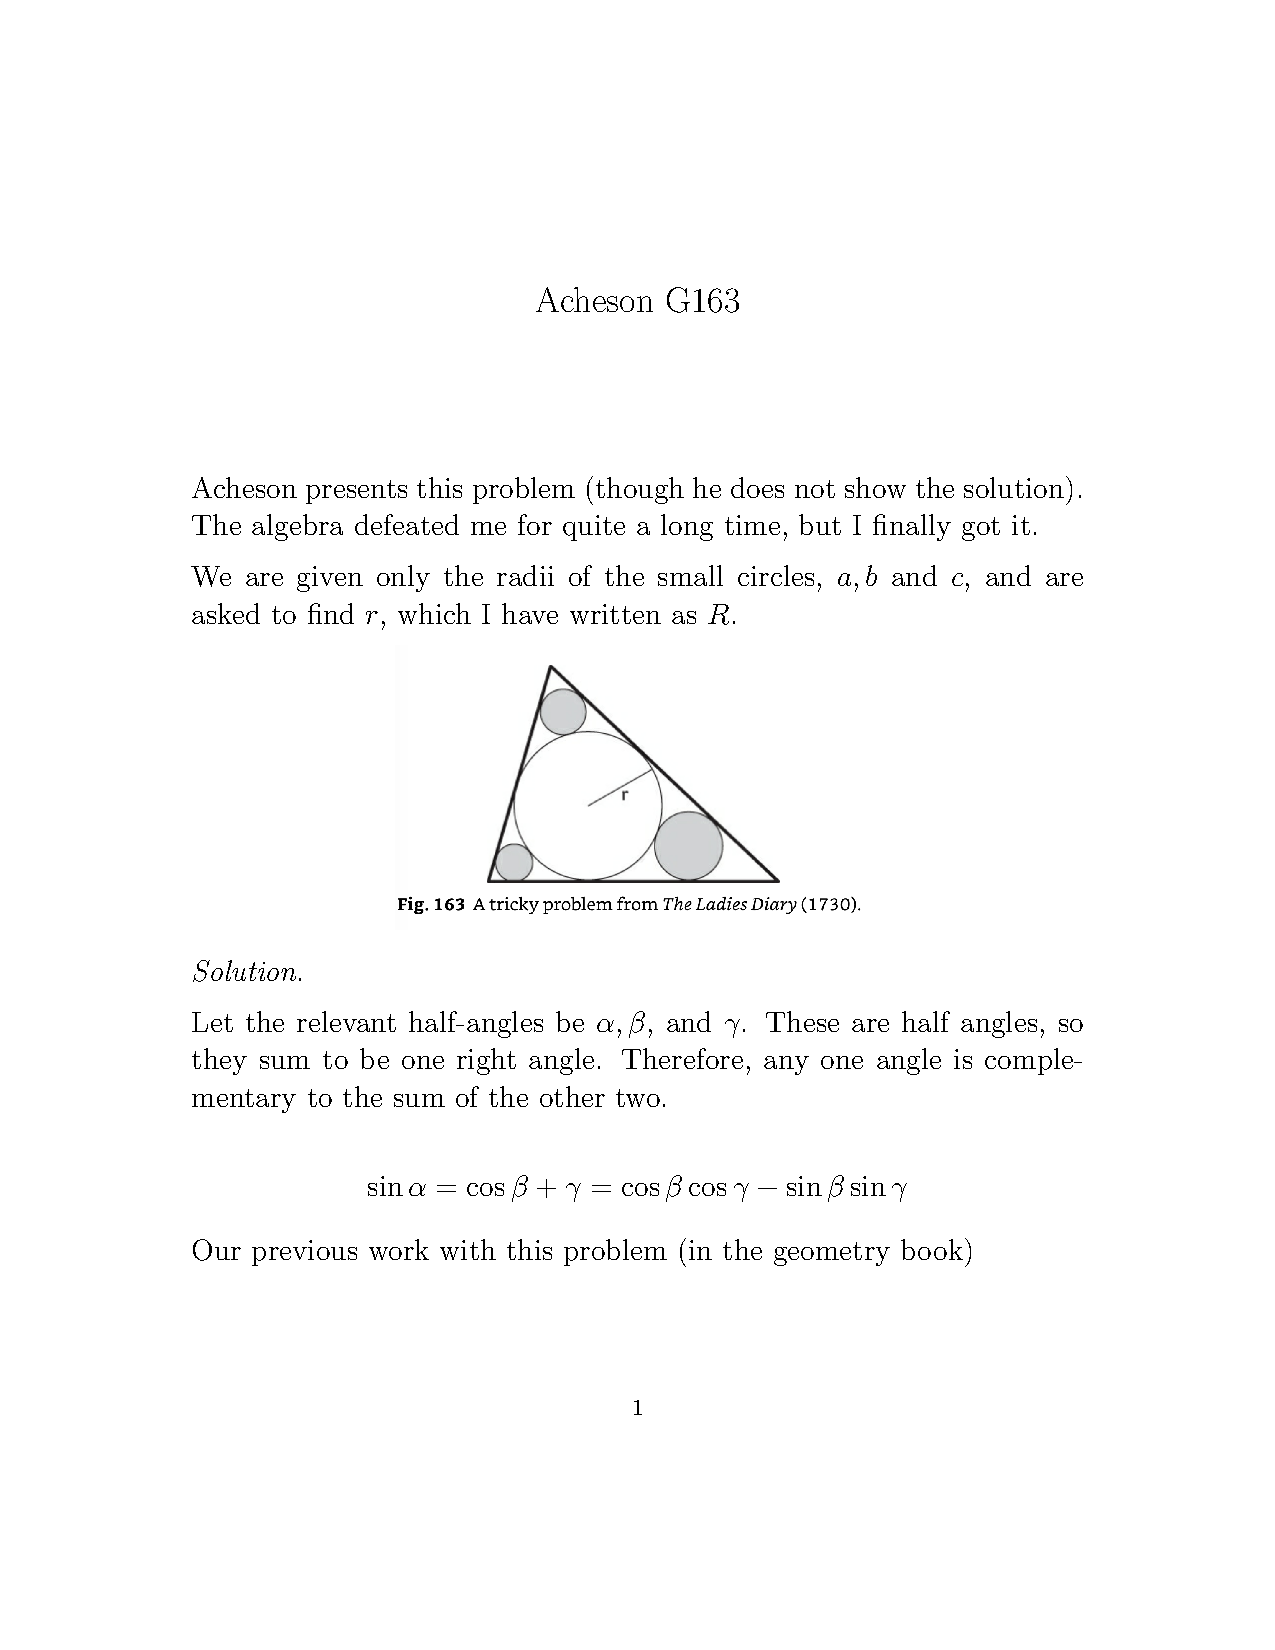
\includegraphics [scale=0.4] {Acheson_G163.png} \end{center}

\emph{Solution}.

Let the relevant half-angles be $\alpha, \beta$, and $\gamma$.  These are half angles, so they sum to be one right angle.  Therefore, any one angle is complementary to the sum of the other two.  

\[ \sin \alpha = \cos \beta + \gamma = \cos \beta \cos \gamma - \sin \beta \sin \gamma \]

Our previous work with this problem (in the geometry book)
\begin{center} \includegraphics [scale=0.5] {double_scoop1.png} \end{center}

showed that 
\[ \sin \theta = \frac{R - r}{R + r}, \ \ \ \ \ \ \cos \theta = \frac{2\sqrt{Rr}}{R + r} \]

Draw similar triangles involving the centers of the two circles to get this result.

We can apply this to the current problem, giving similar formulas for $\alpha$, $\beta$ and $\gamma$ in terms of the radii $a, b$ and $c$ as well as $R$.

So the expression for $\sin \alpha$ above can be written as 
\[ \frac{R - a}{R + a} = \frac{2\sqrt{Rb}}{R + b} \cdot \frac{2\sqrt{Rc}}{R + c} - \frac{R - b}{R + b} \cdot \frac{R - c}{R + c} \]

Rearranging:
\[ (R-a)(R+b)(R+c) + (R+a)(R-b)(R-c) = 4R \sqrt{bc} \cdot (R + a) \]

The first term is
\[ (R-a)(R+b)(R+c) \]
\[ = (R-a)(R^2 + Rb + Rc + bc) \]
\[ = R^3 + R^2b + R^2c + Rbc -R^2a - Rab - Rac - abc \]

The second term is 
\[ (R+a)(R-b)(R-c) \]
\[ = (R+a)(R^2 - Rb - Rc + bc) \]
\[ = R^3 - R^2b - R^2c + Rbc + R^2a - Rab - Rac + abc \]

The sum has four cancelations and four terms remaining:
\[ 2R^3 + 2Rbc - 2Rab - 2Rac =  4R \sqrt{bc} \cdot (R + a) \]

We can factor out $2R$
\[ R^2 + bc - ab - ac =  2 (R + a) \sqrt{bc} \]
\[ R^2 + bc - ab - ac =  2R \ \sqrt{bc} + 2a \sqrt{bc} \]

This is a quadratic in $R$:
\[ R^2 - 2 \sqrt{bc} \ R + bc - ab - ac - 2a \sqrt{bc} \]

The discriminant is
\[ 4bc - 4(bc - ab - ac - 2a \sqrt{bc}) \]

with another cancelation
\[ 4ab + 4ac + 8a \sqrt{bc} \]

The $4$ comes out from the square root as $2$ and we have
\[ R = \frac{2 \sqrt{bc} \pm 2 \sqrt{ab + ac + 2a \sqrt{bc}}}{2} \]
\[ R = \sqrt{bc} \pm \sqrt{ab + ac + 2a \sqrt{bc}} \]

But what is under the square root is a perfect square, namely
\[ ab + ac + 2a \sqrt{bc} = (\sqrt{ab} + \sqrt{ac})^2 \]

We have
\[ R = \sqrt{bc} \pm (\sqrt{ab} + \sqrt{ac}) \]

We will disregard the negative sign and obtain finally
\[ R = \sqrt{bc} + \sqrt{ab} + \sqrt{ac} \]

which is the answer we were given.  As expected, it is symmetric in $a,b$ and $c$.

$\square$


\end{document}